\documentclass[conference,a4paper]{IEEEtran}
\IEEEoverridecommandlockouts

% ---- PACKAGES ----
\usepackage{cite}
\usepackage{amsmath,amssymb,amsfonts}
\usepackage{algorithmic}
\usepackage{graphicx}
\graphicspath{{../figures/}}
\usepackage{textcomp}
\usepackage{xcolor}
\usepackage{gensymb}
\usepackage{booktabs}
\usepackage{hyperref}
\hypersetup{hidelinks}
\usepackage{multirow}
\usepackage{array}
\usepackage{siunitx}
\usepackage{balance}
% ---- Encoding and typography ----
\usepackage{cmap}
\usepackage[T1]{fontenc}
\usepackage{microtype}

\def\BibTeX{{\rm B\kern-.05em{\sc i\kern-.025em b}\kern-.08em
    T\kern-.1667em\lower.7ex\hbox{E}\kern-.125emX}}

% Table row spacing
\renewcommand{\arraystretch}{1.15}

\begin{document}

\title{Substrate-Dependent Performance Variation in Pipe Crack Detection: Diagnosis, Augmentation, and the Limits of Training-Time Mitigation}

\author{
\IEEEauthorblockN{Ma.\ Madecheen S.\ Pangaliman\textsuperscript{1}, Mark Kenneth Biasbas\textsuperscript{2}, Faustino Miguel Flores\textsuperscript{3},\\Carl Christian Gatchalian\textsuperscript{4}, Lorin Angela Velasco\textsuperscript{5}, and Dulce Maria Yadao\textsuperscript{6}}
\IEEEauthorblockA{
\textit{Department of Electronics Engineering} \\
\textit{University of Santo Tomas}\\
Manila, Philippines \\
mspangaliman@ust.edu.ph}
}

\maketitle

% ==============================================================
%   ABSTRACT
% ==============================================================
\begin{abstract}
Automated visual inspection of piping systems is critical for structural integrity monitoring, yet the influence of substrate visual properties on detection performance remains poorly understood. This paper investigates how substrate complexity affects crack detection difficulty when training data quantity is controlled. Three crack specimen categories were fabricated on substrates spanning a texture gradient---smooth PVC to porous tissue---and a class-balanced dataset (400 labels per class) was created. YOLO-World XL and YOLOv8x were fine-tuned across five random seeds on an NVIDIA DGX A100. YOLO-World XL achieved mAP@50-95 of $0.8628 \pm 0.0044$, yet per-class AP ranged from 94.2\% (smooth PVC) to 73.9\% (textured tissue)---a 20.2 percentage point gap consistent across both architectures. Decomposing by IoU threshold reveals this is primarily a \textit{localization} problem: paper crack maintains 97.2\% AP@50 but drops 23.3~pp at stricter thresholds. Three augmentation-based mitigation strategies (CutMix, multi-scale training, and their combination) failed to significantly reduce the gap (Bonferroni-corrected $p > 0.05$), indicating the disparity reflects a fundamental localization challenge tied to substrate visual properties rather than insufficient training-time diversity.
\end{abstract}

\begin{IEEEkeywords}
YOLO-World, object detection, crack detection, pipe inspection, transfer learning, fine-tuning, deep learning, substrate analysis, data augmentation
\end{IEEEkeywords}

% ==============================================================
%   I. INTRODUCTION
% ==============================================================
\section{Introduction}

Structural integrity monitoring of piping systems is a critical safety concern across sectors including oil and gas, water treatment, and manufacturing. Traditional manual inspection methods are labor-intensive, subjective, and often limited to accessible areas. Automated visual inspection systems based on deep learning offer a promising alternative. However, real-world piping systems comprise diverse materials and surface conditions, and the extent to which substrate visual properties influence detection performance remains poorly understood.

The YOLO (You Only Look Once) family \cite{redmon2016yolo} achieves real-time inference by framing detection as a single-stage regression problem. YOLO-World \cite{cheng2024yoloworld} extends this framework with open-vocabulary capabilities through vision-language pre-training, enabling strong transfer learning to custom categories with limited labeled data. These properties make YOLO-World suitable for investigating whether substrate-driven visual differences persist even when training data is controlled, as its pre-trained representations should, in principle, generalize across surface types.

However, a key challenge remains underexplored. Existing studies focus on maximizing overall accuracy or addressing class imbalance through oversampling and augmentation, implicitly assuming that balanced training data yields comparable per-class performance. In practice, pipe cracks occur on surfaces with diverse textures, yet the relationship between substrate visual complexity and detection performance has not been systematically investigated \cite{hsieh2020crack, liu2023survey}. While recent work on texture-aware defect detection \cite{li2024texmsyolo} has shown that background complexity degrades performance, that work evaluated a single surface type without controlling for class balance, leaving open the question of whether such effects persist when training data quantity is explicitly equalized across substrates.

This paper addresses the following research question: \textbf{How does the visual complexity of the defect substrate affect detection performance when training data quantity is controlled and balanced?} We designed a controlled experiment using three crack specimen categories, each with exactly 400 annotated labels, spanning a range of substrate texture from smooth PVC to porous tissue. The contributions are fourfold:

\begin{enumerate}
    \item A controlled experiment examining how defect-substrate visual properties affect detection difficulty by holding training data constant at 400 labels per class.
    \item Quantitative evidence, under controlled and class-balanced conditions, that defect-substrate visual properties produce a 20--22 percentage point per-class AP gap---an effect consistent across both YOLO-World XL and YOLOv8x over five random seeds and not reducible to data imbalance.
    \item An evaluation of three augmentation-based mitigation strategies (CutMix, multi-scale training, and their combination), providing evidence on whether standard training-time augmentation can close the substrate-dependent performance gap.
    \item A publicly available class-balanced dataset and multi-seed evaluation protocol that enable independent replication and extension of substrate-dependent detection experiments.
\end{enumerate}

% ==============================================================
%   II. RELATED WORK
% ==============================================================
\section{Related Work}

\subsection{Crack Detection Methods}

Crack detection has been extensively studied in civil infrastructure \cite{hsieh2020crack}. Early approaches relied on edge detection and morphological operations; with the advent of deep learning, CNN-based methods have largely superseded them \cite{liu2023survey}. Cha et al.\ \cite{cha2017deep} demonstrated a CNN-based crack detector achieving 98\% accuracy on concrete surfaces. For pipe inspection, Lv et al.\ \cite{li2024sewer} proposed a lightweight YOLOv8n method deployed on an amphibious sewer robot. However, these studies evaluate detection performance in aggregate across a single surface type, without examining how substrate properties affect per-class difficulty.

\subsection{YOLO-Based Object Detection}

The YOLO architecture \cite{redmon2016yolo} frames detection as single-stage regression. Successive iterations through YOLOv8 \cite{jocher2023ultralytics} have improved accuracy via feature pyramid networks, anchor-free heads, and advanced loss functions. YOLO-World \cite{cheng2024yoloworld} further extends this paradigm with a Re-parameterizable Vision-Language Path Aggregation Network (RepVL-PAN) that enables open-vocabulary detection by aligning visual and textual representations through CLIP \cite{radford2021clip} text embeddings. This vision-language fusion is designed to generalize across visual domains, making it well-suited for examining whether substrate-dependent performance gaps persist even with a highly generalizable detector.

\subsection{Data Augmentation for Hard Examples}

CutMix \cite{yun2019cutmix} generates composite training images by replacing rectangular patches with regions from other samples and mixing the corresponding labels, encouraging the detector to attend to discriminative local features rather than global context. Multi-scale training varies the input resolution across iterations, exposing the model to objects at diverse scales and improving robustness to size variation. Both techniques are standard in modern object detection pipelines and impose no additional annotation cost. Copy-paste augmentation \cite{ghiasi2021copypaste} offers stronger instance-level diversity but requires segmentation masks, making it inapplicable to bounding-box-only datasets such as ours. We therefore evaluate CutMix and multi-scale training---individually and in combination---as practical, mask-free strategies for closing the substrate-dependent AP gap.

\subsection{Transfer Learning for Industrial Inspection}

Pre-trained models on large-scale datasets such as COCO \cite{lin2014coco} and Objects365 \cite{shao2019objects365} provide robust features adaptable to specialized tasks. However, while class imbalance \cite{japkowicz2023class} and its effects on object detection \cite{oksuz2021imbalance} have been studied extensively, per-class performance variation driven by differences in visual properties---rather than data quantity---remains underexplored. Our work addresses this gap for pipe crack detection on substrates of varying complexity, comparing both an open-vocabulary (YOLO-World XL) and a standard (YOLOv8x) detector under identical conditions.

% ==============================================================
%   III. METHODOLOGY
% ==============================================================

\section{Methodology}

Building on the gaps identified in the literature, this section describes the experimental design used to examine how defect-substrate visual properties affect detection difficulty under controlled data conditions.

\subsection{Dataset Preparation}

Three categories of crack specimens were fabricated under controlled laboratory conditions on blue-colored substrates, serving as controlled proxies that span a visual complexity gradient from idealized defects on smooth surfaces to realistic crack patterns on textured, porous materials: (1)~\textit{dummy cracks}---lines drawn on smooth PVC pipes, producing sharp, high-contrast patterns; (2)~\textit{PVC pipe cracks}---physical fractures on smooth PVC, introducing genuine but irregular crack geometry; and (3)~\textit{paper cracks}---cracks on blue-painted tissue rolls, where the porous substrate creates a noisy background that obscures crack edges. By keeping the number of training labels identical across all three types, any observed performance differences can be attributed to differences in defect-substrate visual properties---including both substrate texture and crack morphology---rather than unequal training effort.

To control for data quantity as a confounding factor, the dataset was designed to be strictly class-balanced, comprising exactly 400 annotated bounding box labels per class (1,200 total), annotated using Roboflow \cite{roboflow2023}. Preprocessing included auto-orientation, resizing to $640 \times 640$ pixels, and contrast adjustment. Data augmentation ($3\times$ multiplier) comprised flips, rotation ($\pm15\degree$), shear ($\pm10\degree$), brightness ($\pm25\%$), exposure ($\pm15\%$), blur (up to 1.5\,px), and noise (up to 1\%). Grayscale conversion, hue shifts, and random cropping were excluded from offline preprocessing to preserve crack features; standard Ultralytics online augmentation (mosaic, mixup) was applied identically to all classes during training.

The augmented dataset (2,617 images) was split into training (88\%, 2,292), validation (8\%, 217), and test (4\%, 108). Table~\ref{tab:dataset} summarizes the composition. Fig.~\ref{fig:samples} shows annotated samples from each class.

\begin{table}[htbp]
\caption{Dataset Composition and Split Configuration}
\begin{center}
\begin{tabular*}{\columnwidth}{@{\extracolsep{\fill}}lc}
\toprule
\textbf{Property} & \textbf{Value} \\
\midrule
Labels per class (Dummy / Paper / PVC) & 400 / 400 / 400 \\
Total annotations           & 1,200 \\
Post-augmentation images    & 2,617 \\
\midrule
Training set                & 2,292 (88\%) \\
Validation set              & 217 (8\%) \\
Test set                    & 108 (4\%) \\
\bottomrule
\end{tabular*}
\label{tab:dataset}
\end{center}
\end{table}

\begin{figure}[htbp]
\centerline{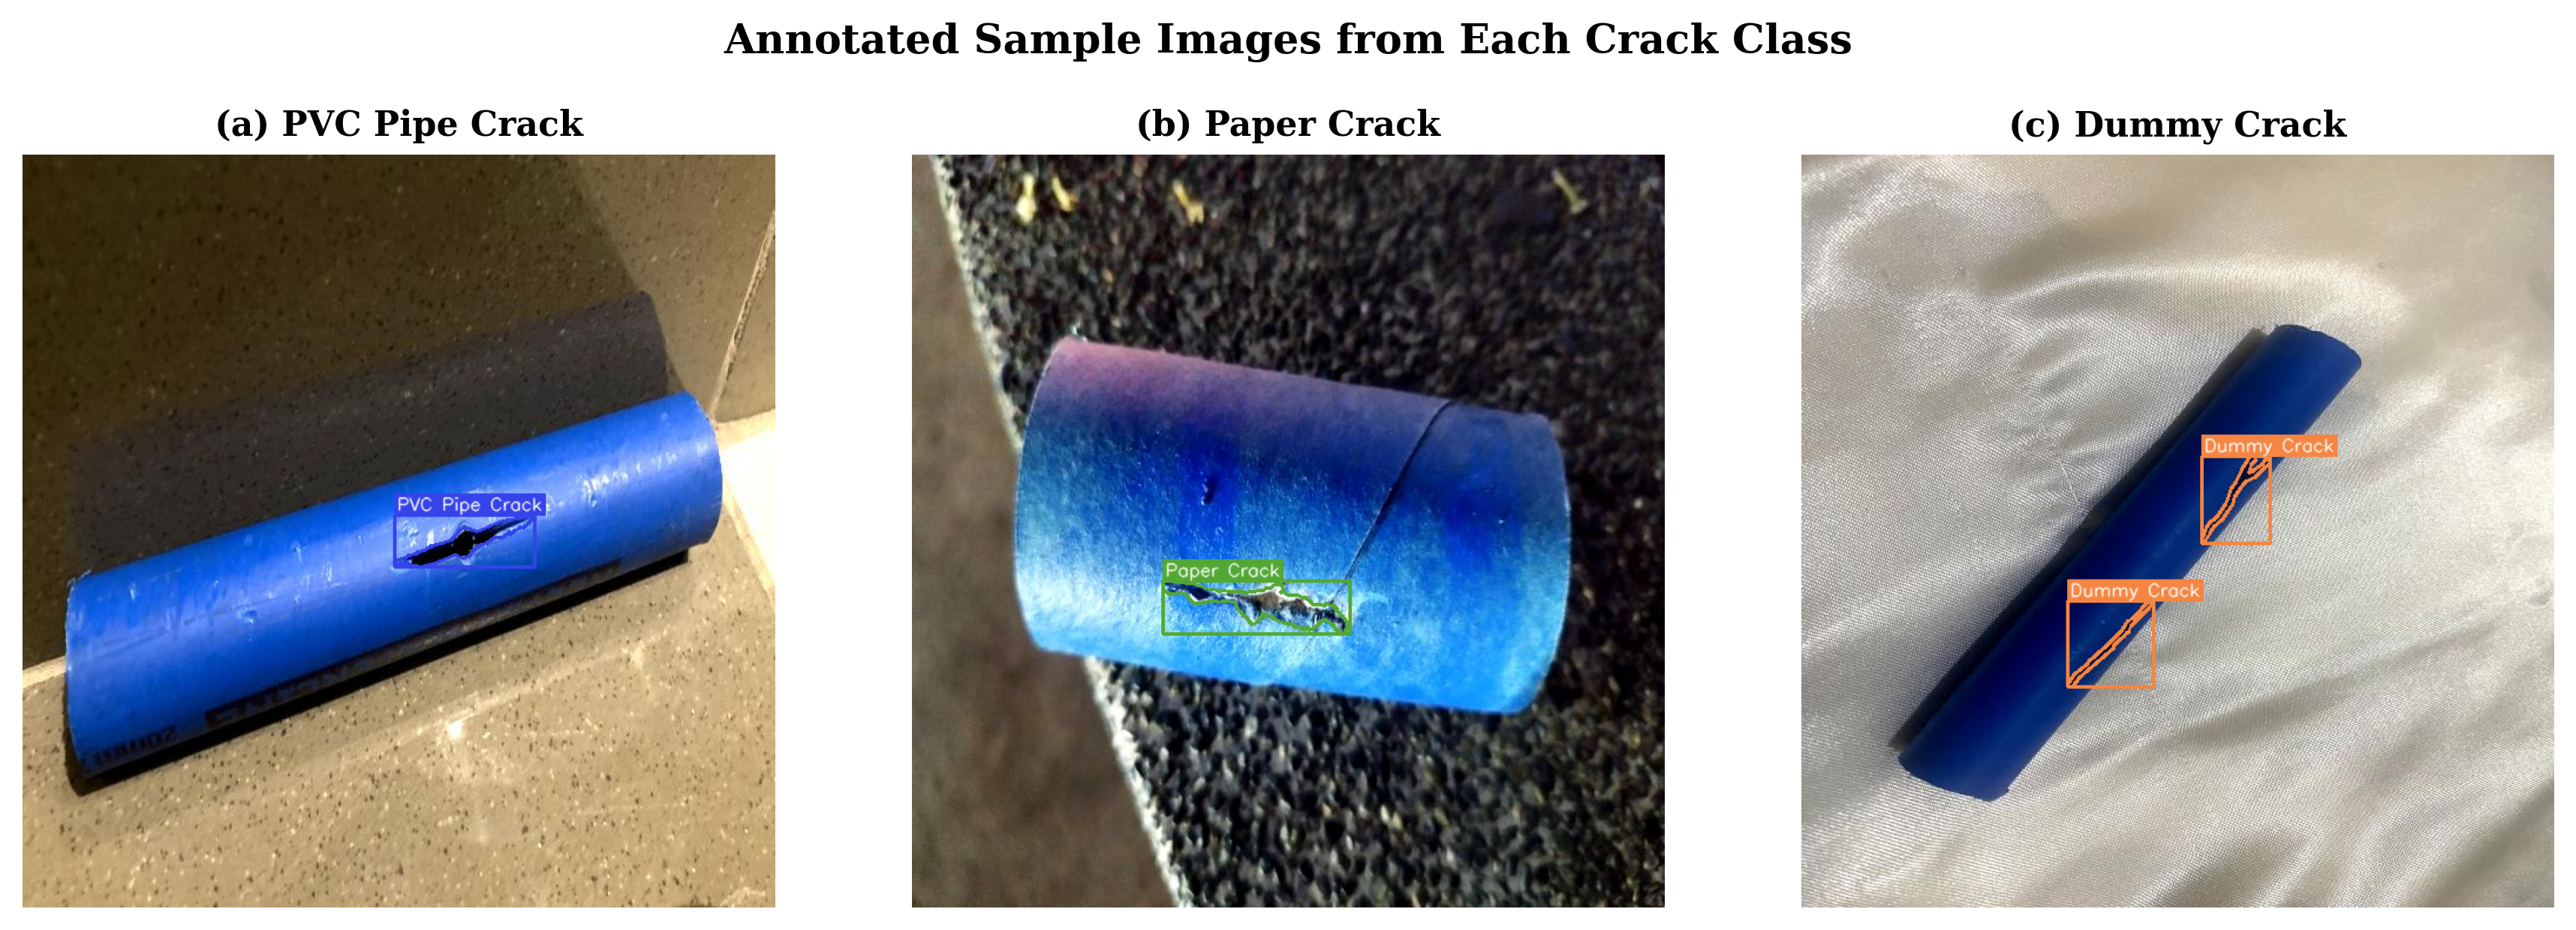
\includegraphics[width=\columnwidth]{fig_samples.png}}
\caption{Annotated samples with ground-truth bounding boxes. (a)~PVC pipe crack. (b)~Paper crack. (c)~Dummy crack.}
\label{fig:samples}
\end{figure}

\subsection{Model Architecture}

YOLO-World XL (YOLOv8x-worldv2) was selected as the detection backbone, comprising 127 layers, 72,856,217 parameters, and 273.3 GFLOPs. The architecture extends YOLOv8 \cite{jocher2023ultralytics} with a RepVL-PAN that fuses visual features with CLIP \cite{radford2021clip} text embeddings. The XL variant was chosen to maximize detection capacity, ensuring that any observed per-class performance differences reflect substrate complexity rather than model capacity limitations. The YOLOv8 backbone was pre-trained on COCO \cite{lin2014coco}, and the YOLO-World model was subsequently trained on Objects365 \cite{shao2019objects365} and GoldG grounding data, providing diverse visual priors that should, in principle, support detection across all three substrate types.

\subsection{Training Configuration}

Fine-tuning was performed on an NVIDIA DGX A100-40GB for 100 epochs using AdamW \cite{loshchilov2019adamw} with a learning rate of $2 \times 10^{-4}$, weight decay of 0.05, batch sizes of 8 (YOLO-World XL) and 16 (YOLOv8x)---with Ultralytics' nominal batch size ($\mathrm{nbs}=64$) auto-scaling the effective learning rate---and $640 \times 640$ input resolution. All three crack classes were trained jointly under identical conditions, with no class-specific learning rates, loss weights, or augmentation strategies, ensuring that any observed per-class differences are attributable to defect-substrate visual properties rather than training procedure variations. Early stopping patience was set to 20 epochs, and the best model was selected by validation mAP@50-95. To assess statistical reliability, both YOLO-World XL and a standard YOLOv8x baseline were trained five times each with different random seeds (0, 1, 2, 42, 123) under identical hyperparameters. The dataset splits were held fixed across all 10 runs (5 seeds $\times$ 2 models); only weight initialization and stochastic training operations varied. The low standard deviations observed (std $\leq 0.014$ across all metrics and classes) confirm stable optimization; all runs converged without overfitting. Experiment tracking used Weights \& Biases \cite{biewald2020wandb}.

\subsection{Evaluation Metrics}

Detection performance is evaluated following the COCO protocol \cite{lin2014coco} using precision, recall, F1 score, and mean Average Precision (mAP). The primary metric is mAP@50-95, which averages AP across ten IoU thresholds from 0.50 to 0.95, penalizing imprecise localization more heavily than mAP@50 and making it more sensitive to the substrate-dependent bounding box quality differences under investigation.

\subsection{Mitigation Strategies}

To test whether standard augmentation can reduce the substrate-dependent AP gap, three strategies were applied to YOLO-World XL only, keeping all other hyperparameters identical to the baseline:

\begin{enumerate}
    \item \textbf{CutMix} \cite{yun2019cutmix}: rectangular patches from other training images are pasted onto each sample with probability 0.5 (\texttt{cutmix=0.5}), encouraging the model to learn from partial crack evidence and diverse background context.
    \item \textbf{Multi-scale training}: the input resolution is randomly varied around $960 \times 960$ during training (\texttt{multi\_scale=True}), while evaluation remains at $640 \times 640$ for fair comparison. This exposes the model to crack patterns at multiple scales, potentially improving localization on textured substrates.
    \item \textbf{Combined}: CutMix and multi-scale training are applied together.
\end{enumerate}

Each strategy was trained with the same five seeds as the baseline for paired comparison. The batch size was reduced from 8 to 4 for multi-scale and combined strategies to prevent out-of-memory errors at the higher training resolution; Ultralytics' nominal batch size mechanism ($\mathrm{nbs}=64$) automatically scales the effective learning rate, keeping optimization dynamics matched across configurations.

% ==============================================================
%   IV. EXPERIMENTAL RESULTS
% ==============================================================

\section{Experimental Results}

Having established the controlled experimental design, this section presents both aggregate and per-class detection results to assess whether substrate complexity produces measurable performance differences.

\subsection{Overall and Per-Class Performance}

For the best single run (seed~42), YOLO-World XL achieves an overall mAP@50-95 of 0.8692 on the test set. However, per-class results (Table~\ref{tab:perclass}) reveal substantial variation: dummy crack achieves AP@50-95 of 0.9560, followed by PVC pipe crack at 0.9116 and paper crack at 0.7400---a 21.6 percentage point gap despite 400 labels per class. We note that the test set contains 108 images (${\sim}$36 per class); while the multi-seed design controls for training stochasticity, per-class AP estimates carry sampling uncertainty that larger test sets would reduce. Multi-seed averages in Section~\ref{sec:model_comparison} confirm a consistent 20--22~pp gap across both architectures.

\begin{table}[htbp]
\caption{Per-Class Average Precision (Best Single Run, Test Set)}
\begin{center}
\begin{tabular*}{\columnwidth}{@{\extracolsep{\fill}}lcccc}
\toprule
\textbf{Class} & \textbf{AP@50-95} & \textbf{Prec.} & \textbf{Recall} & \textbf{Train Labels} \\
\midrule
Dummy crack    & \textbf{0.9560} & 0.987 & \textbf{0.988} & 400 \\
PVC pipe crack & 0.9116          & \textbf{0.989} & 0.938 & 400 \\
Paper crack    & 0.7400          & 0.986 & 0.963 & 400 \\
\bottomrule
\end{tabular*}
\label{tab:perclass}
\end{center}
\end{table}

This hierarchy aligns with the substrate complexity gradient described in Section~III-A and is consistent with the expectation that textured backgrounds reduce detection confidence by obscuring crack edges. Fig.~\ref{fig:qualitative} shows representative detection outputs: bounding boxes on dummy and PVC pipe cracks are tight and well-defined, whereas paper crack predictions exhibit visibly looser localization, consistent with the 23.3~pp gap between AP@50 and AP@50-95 analyzed in Section~V-A.

\begin{figure}[htbp]
\centerline{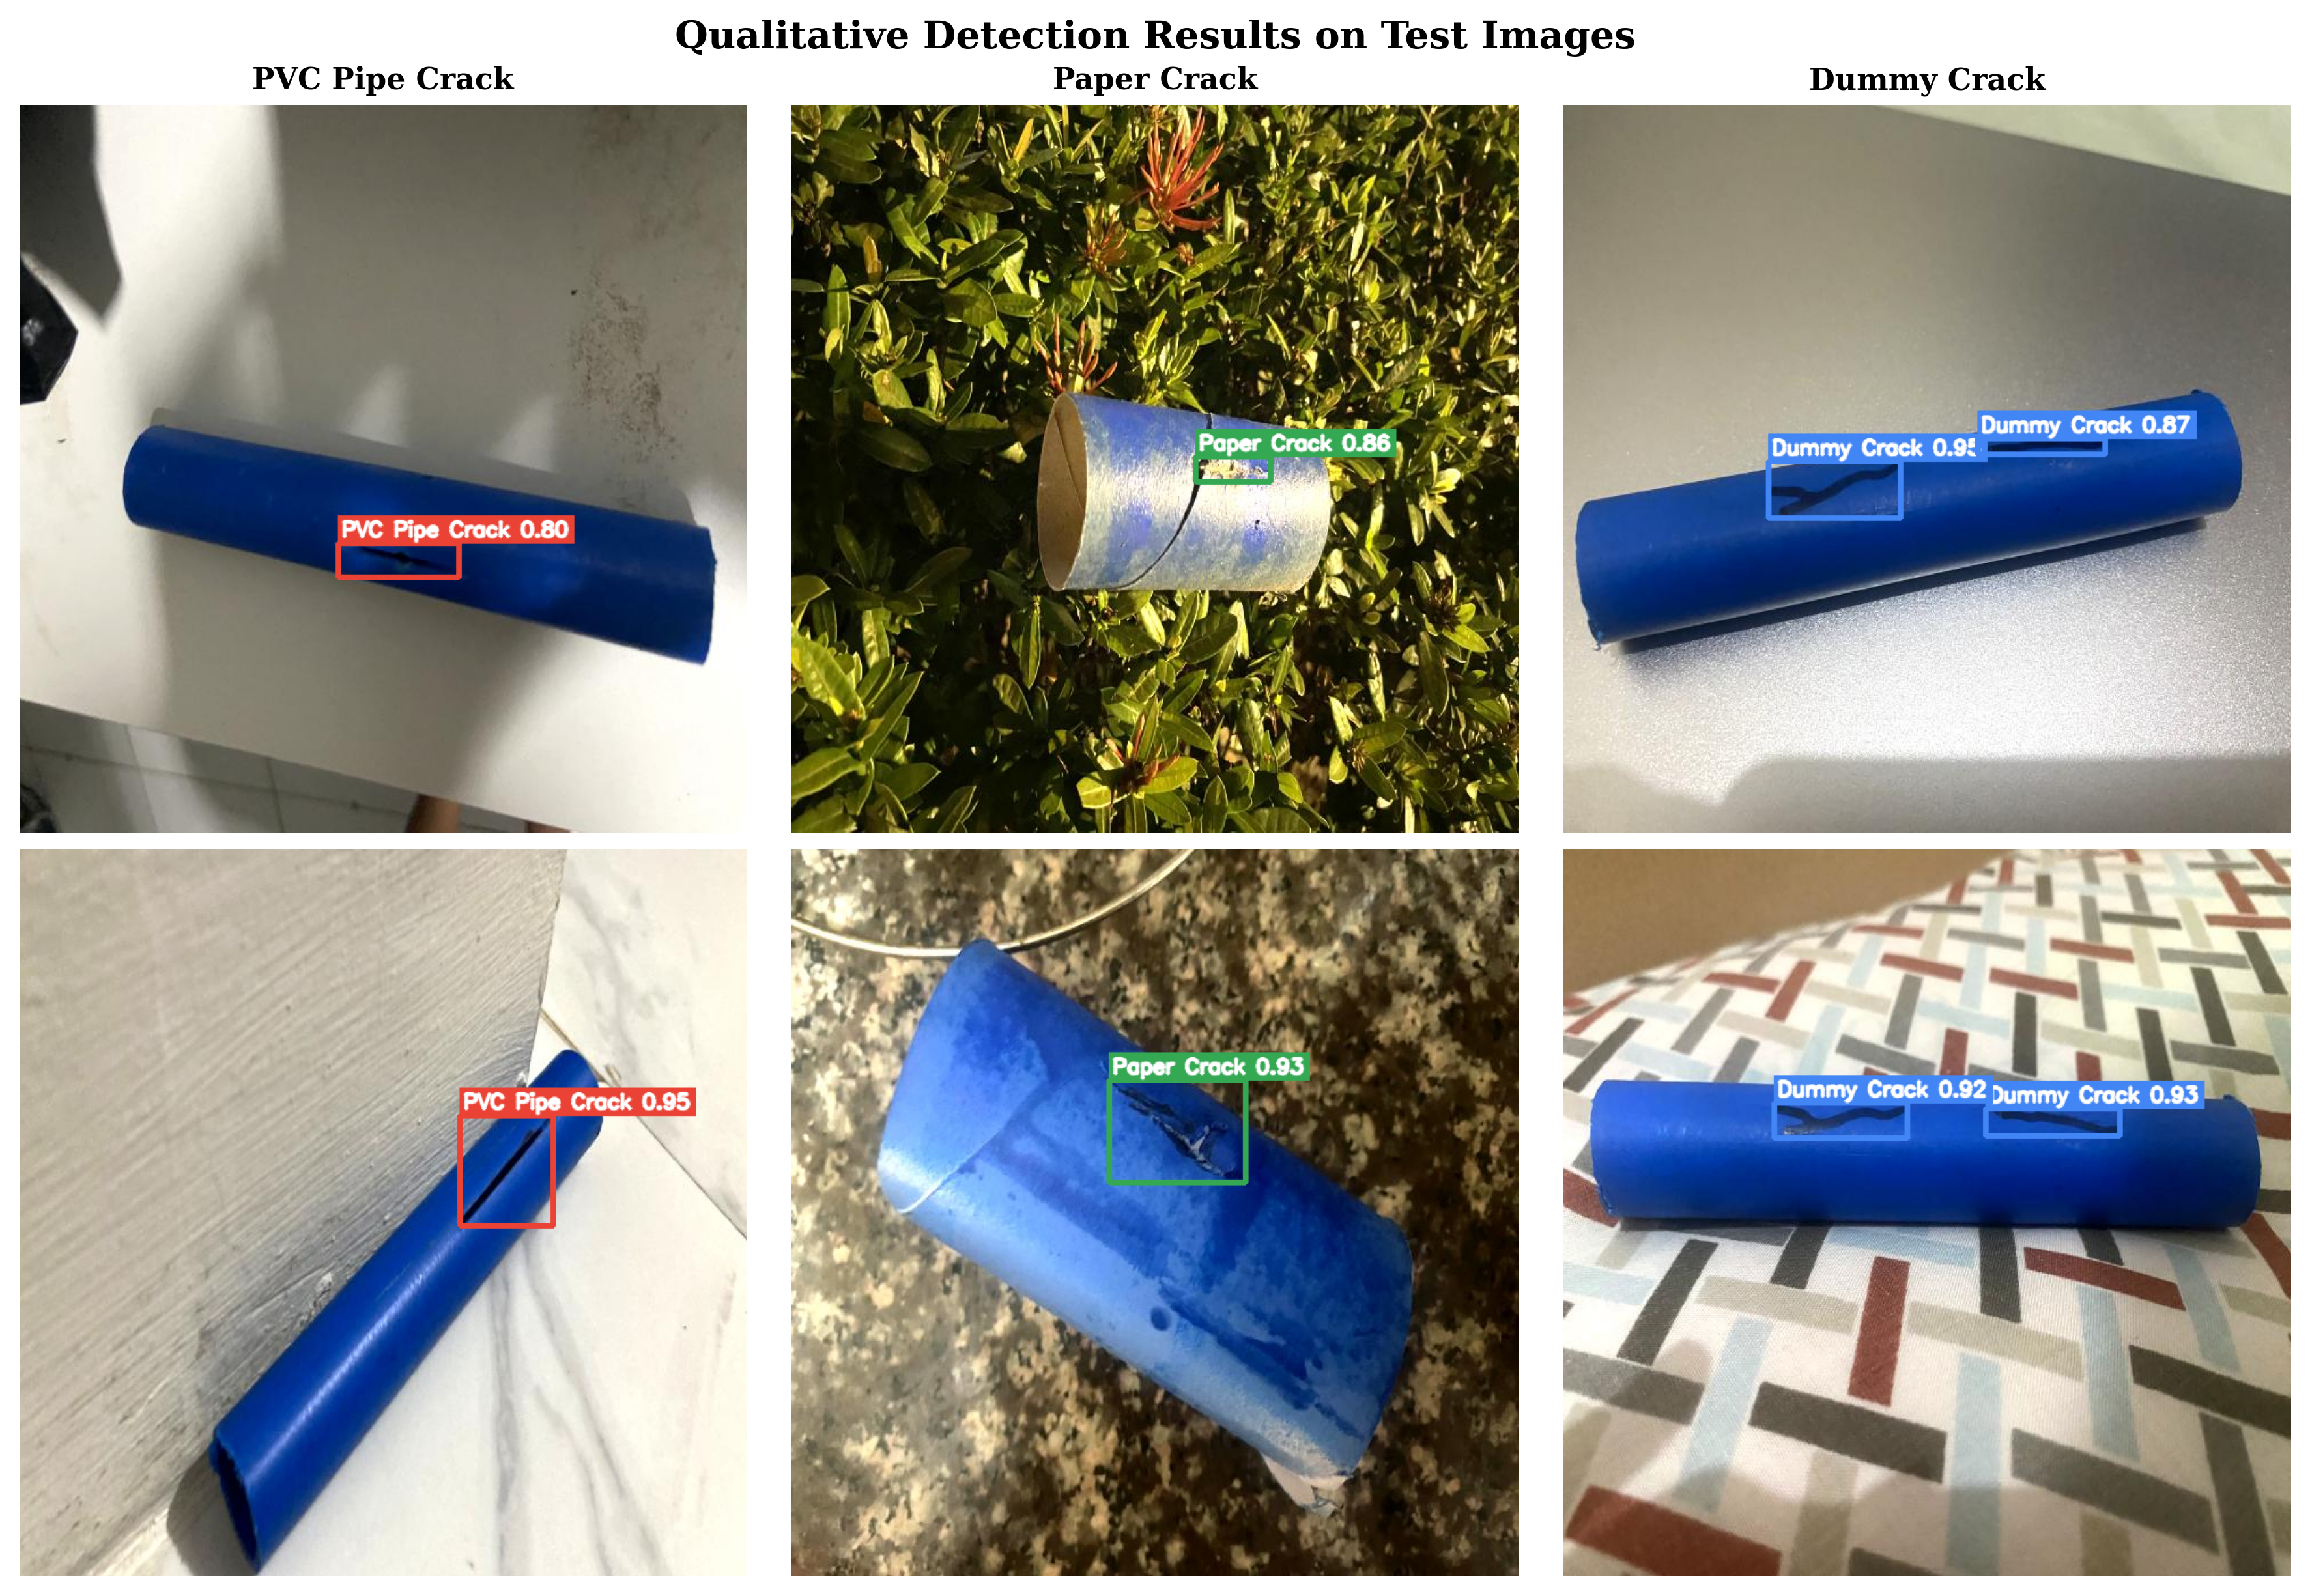
\includegraphics[width=\columnwidth]{fig_qualitative.png}}
\caption{Qualitative detection results from YOLO-World XL (best run, seed~42). Bounding boxes on dummy and PVC pipe cracks are tight, whereas paper crack predictions show visibly looser localization where crack edges blend into the textured substrate.}
\label{fig:qualitative}
\end{figure}

\subsection{Model Comparison: YOLO-World XL vs.\ YOLOv8x}
\label{sec:model_comparison}

To determine whether the substrate-dependent performance gap is specific to YOLO-World or consistent across architectures, both YOLO-World XL and a standard YOLOv8x model (without open-vocabulary capability) were trained under identical conditions across five random seeds. Although both share a YOLOv8 backbone, they differ substantively: YOLO-World XL incorporates a CLIP text encoder and RepVL-PAN for vision-language fusion (${\sim}$72.9M parameters), whereas YOLOv8x uses standard detection heads without language grounding (${\sim}$68.2M parameters). Table~\ref{tab:model_comparison} summarizes the results. Statistical significance is assessed using a paired $t$-test with observations paired by seed over the fixed test set.

\begin{table}[htbp]
\caption{YOLO-World XL vs.\ YOLOv8x on the Test Set (Mean $\pm$ Std, 5 Seeds)}
\begin{center}
\begin{tabular*}{\columnwidth}{@{\extracolsep{\fill}}lcccc}
\toprule
\textbf{Metric} & \textbf{YOLO-World XL} & \textbf{YOLOv8x} & $\boldsymbol{p}$ & $\boldsymbol{d}$ \\
\midrule
mAP@50-95  & $\mathbf{0.8628 \pm 0.0044}$ & $0.8545 \pm 0.0075$ & $0.124$ & $1.35$ \\
mAP@50     & $\mathbf{0.9862 \pm 0.0019}$ & $0.9807 \pm 0.0056$ & $0.038^{*}$ & $1.31$ \\
Precision  & $\mathbf{0.9849 \pm 0.0040}$ & $0.9787 \pm 0.0072$ & $0.157$ & $1.06$ \\
Recall     & $\mathbf{0.9803 \pm 0.0047}$ & $0.9686 \pm 0.0109$ & $0.024^{*}$ & $1.40$ \\
F1 Score   & $\mathbf{0.9826 \pm 0.0040}$ & $0.9736 \pm 0.0079$ & $0.025^{*}$ & $1.44$ \\
\midrule
\multicolumn{5}{l}{\textit{Per-class AP@50-95}} \\
\midrule
Dummy crack     & $\mathbf{0.9415 \pm 0.0096}$ & $0.9396 \pm 0.0084$ & --- & --- \\
PVC pipe crack  & $\mathbf{0.9077 \pm 0.0047}$ & $0.8996 \pm 0.0140$ & --- & --- \\
Paper crack     & $\mathbf{0.7393 \pm 0.0067}$ & $0.7243 \pm 0.0134$ & --- & --- \\
\bottomrule
\multicolumn{5}{l}{\footnotesize $^{*}p < 0.05$ (paired $t$-test, $n=5$ seeds). $d$: Cohen's $d$ (pooled SD).} \\
\multicolumn{5}{l}{\footnotesize Per-class statistics omitted due to insufficient power at $n=5$.} \\
\end{tabular*}
\label{tab:model_comparison}
\end{center}
\end{table}

\begin{figure}[htbp]
\centerline{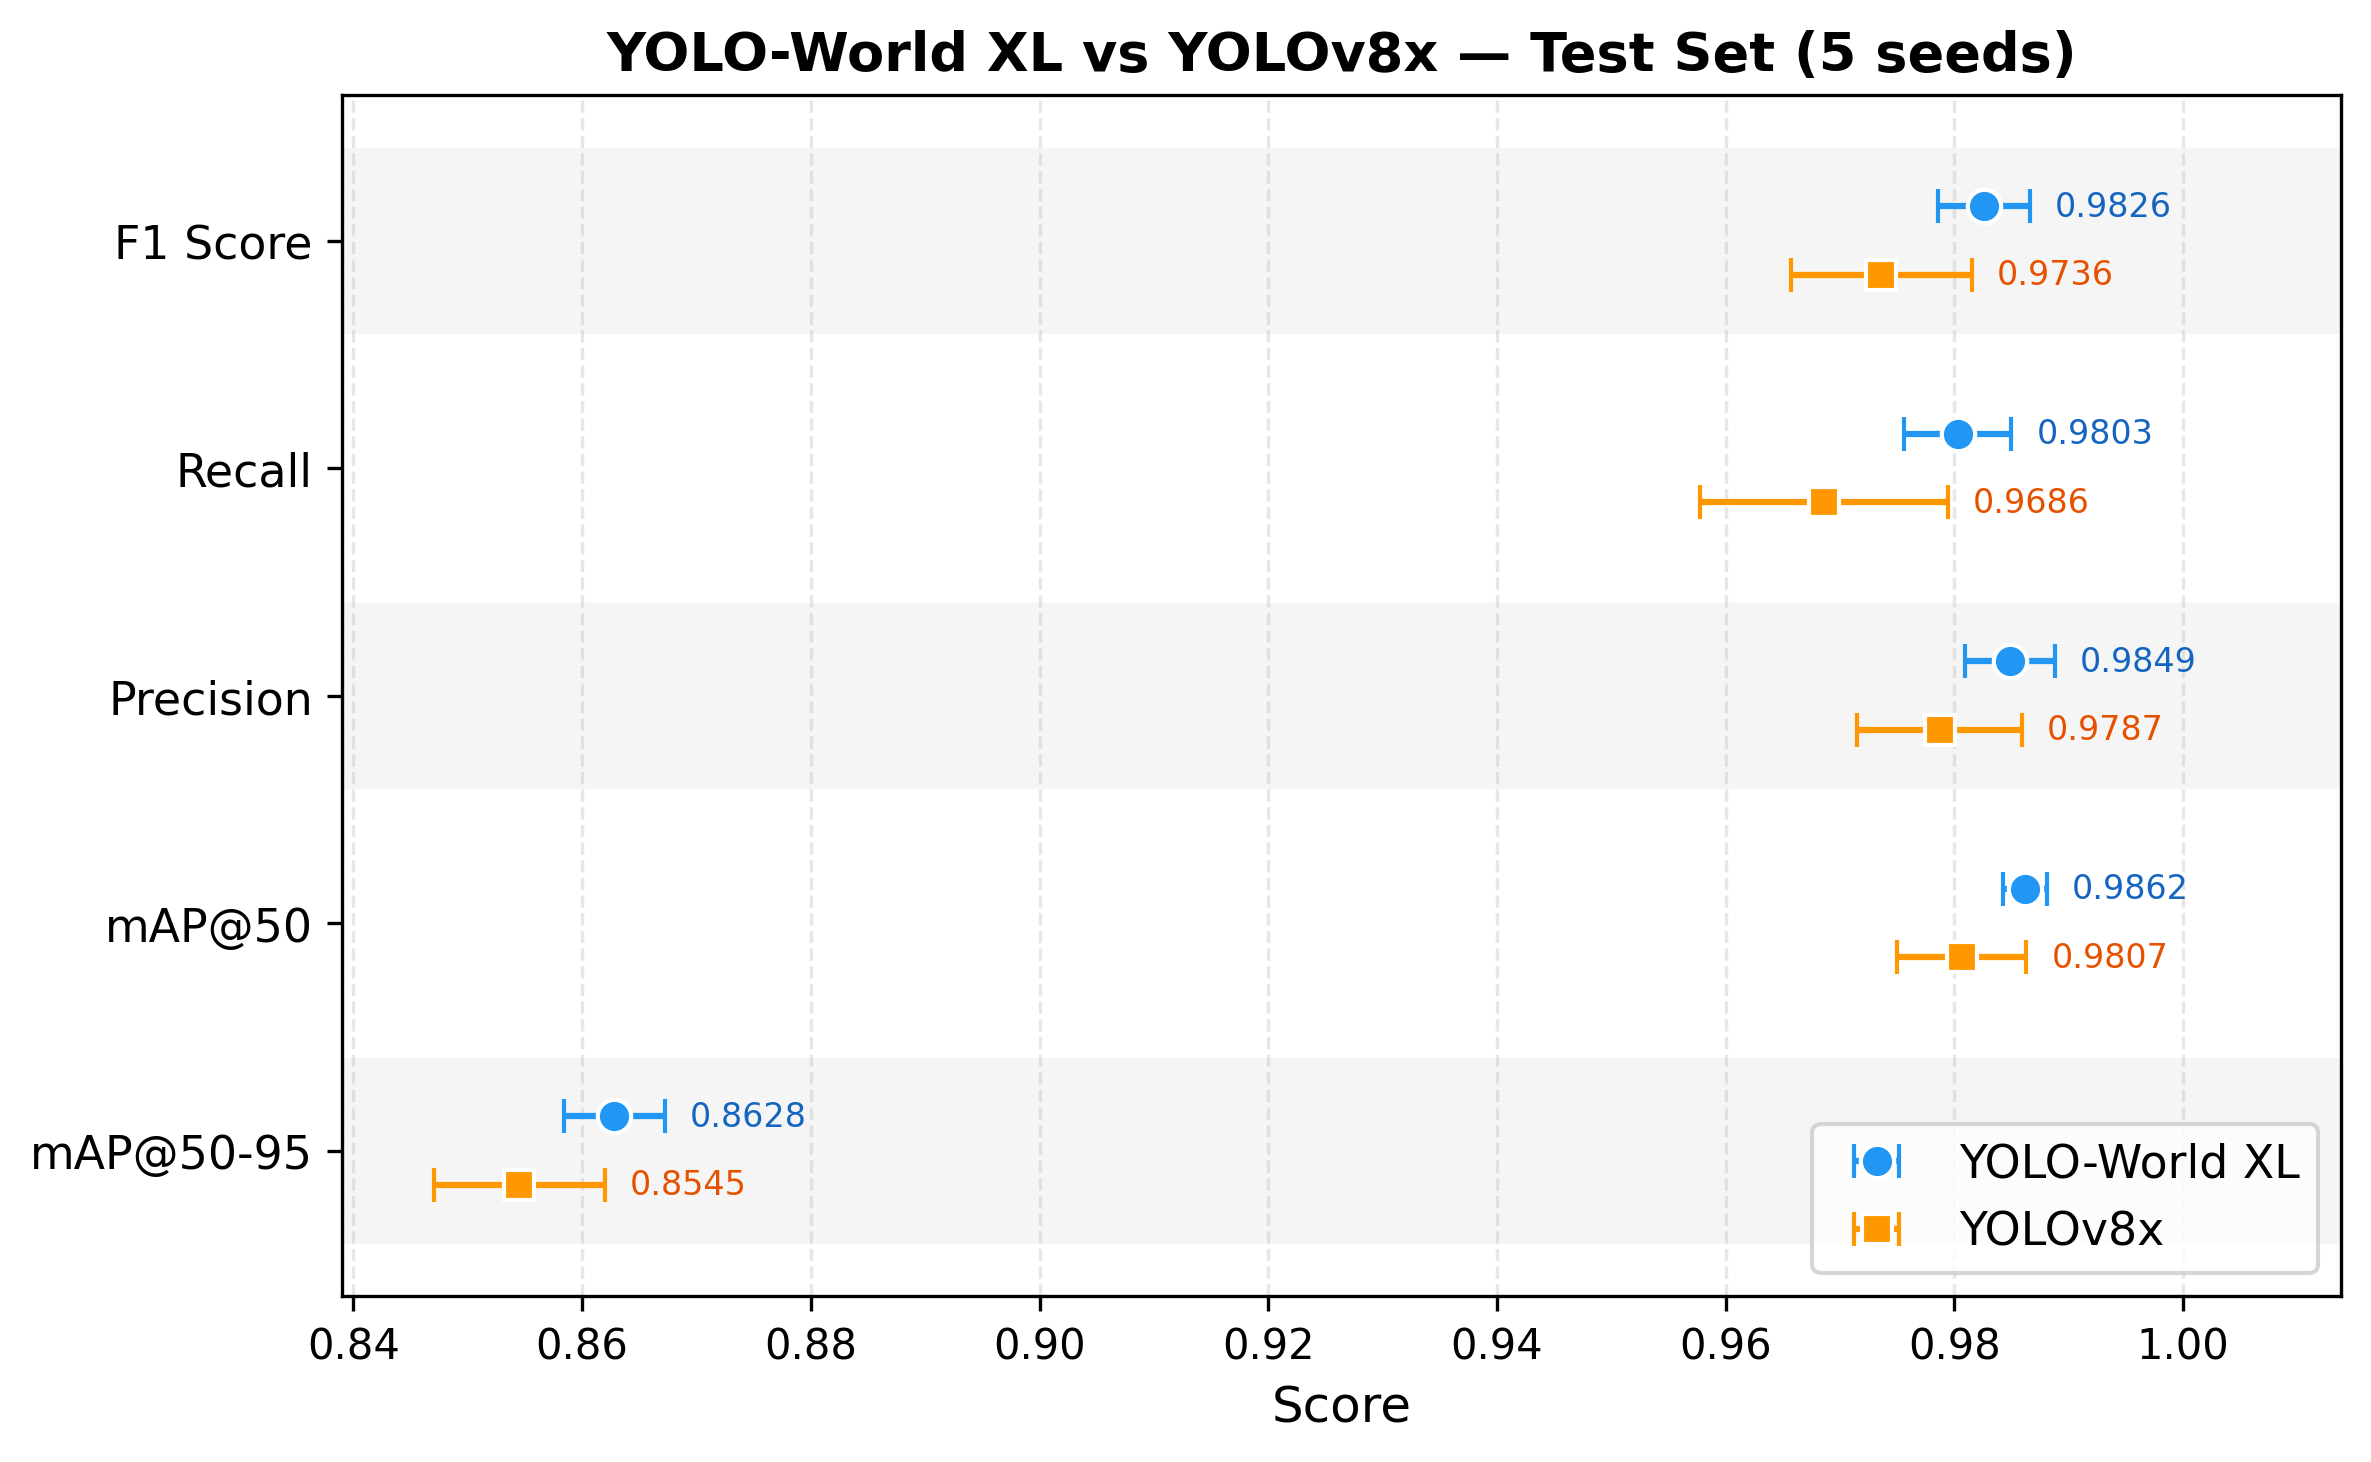
\includegraphics[width=\columnwidth]{fig_model_comparison.png}}
\caption{YOLO-World XL vs.\ YOLOv8x on the test set (mean $\pm$ std, 5 seeds). YOLO-World XL outperforms across all metrics with lower variance.}
\label{fig:model_comparison}
\end{figure}

YOLO-World XL outperforms YOLOv8x across all metrics (Table~\ref{tab:model_comparison}, Fig.~\ref{fig:model_comparison}). A paired $t$-test confirms that improvements in mAP@50 ($p=0.038$), recall ($p=0.024$), and F1 ($p=0.025$) are statistically significant at the 5\% level. The mAP@50-95 gain ($+0.83$~pp) trends in the same direction but does not reach significance ($p=0.124$). Cohen's $d$ values range from 1.06 to 1.44 across all aggregate metrics, indicating large practical effects regardless of statistical significance at $n=5$. YOLO-World XL exhibits roughly half the variance of YOLOv8x, possibly reflecting differences in pre-training or model capacity. The per-class hierarchy is preserved in both architectures: the AP gap between dummy crack and paper crack is 20.2~pp for YOLO-World XL and 21.5~pp for YOLOv8x, confirming that the substrate complexity effect is consistent across both detector architectures tested.

Regarding inference speed, YOLO-World XL incurs a 24\% latency overhead (21.2\,ms vs.\ 17.1\,ms inference on an A100 at $640 \times 640$) due to its CLIP text encoder, but both models comfortably exceed real-time frame rates (37.6 and 42.0 FPS, respectively).

\subsection{Mitigation Strategy Evaluation}
\label{sec:mitigation}

Table~\ref{tab:mitigation} compares the three augmentation-based mitigation strategies against the YOLO-World XL baseline on the test set, with statistical significance assessed via paired $t$-tests (by seed) and Bonferroni correction ($\alpha = 0.05/3 \approx 0.0167$). Fig.~\ref{fig:mitigation} visualizes per-class AP and the substrate gap across strategies.

None of the three strategies improved overall detection performance relative to the baseline: CutMix reduced mAP@50-95 by 2.3~pp ($0.8628 \to 0.8399$, $p=0.085$), Multi-Scale by 2.4~pp ($0.8628 \to 0.8390$, $p=0.147$), and Combined by 5.8~pp ($0.8628 \to 0.8045$, $p=0.115$). None of these differences reach statistical significance after Bonferroni correction.

Regarding the substrate gap (Dummy crack AP minus Paper crack AP), the baseline gap of 20.2~pp was not significantly reduced by any strategy. Multi-Scale achieved the largest reduction ($20.2 \to 18.1$~pp, $\Delta=-2.1$~pp, $p=0.334$), while CutMix slightly increased it ($20.2 \to 21.2$~pp, $\Delta=+1.0$~pp, $p=0.562$). The Combined strategy reduced the gap to 18.4~pp ($\Delta=-1.8$~pp, $p=0.102$), but at the cost of substantially degraded overall performance and increased variance (std$=0.0657$ vs.\ baseline std$=0.0044$). Table~\ref{tab:mitigation} summarises the full results; Fig.~\ref{fig:mitigation} visualizes per-class AP and the substrate gap.

\begin{table}[ht]
\centering
\caption{Mitigation strategy evaluation on the test set (mean $\pm$ std, 5 seeds). Strategies applied to YOLO-World XL only.}
\label{tab:mitigation}
\begin{tabular}{lcccc}
\toprule
Metric & Baseline & CutMix & Multi-Scale & Combined \\
\midrule
mAP@50-95 & \textbf{$0.8628 \pm 0.0044$} & $0.8399 \pm 0.0218$ & $0.8390 \pm 0.0284$ & $0.8045 \pm 0.0657$ \\
mAP@50 & \textbf{$0.9862 \pm 0.0019$} & $0.9852 \pm 0.0025$ & $0.9786 \pm 0.0081$ & $0.9570 \pm 0.0506$ \\
Precision & \textbf{$0.9849 \pm 0.0040$} & $0.9792 \pm 0.0081$ & $0.9718 \pm 0.0111$ & $0.9506 \pm 0.0458$ \\
Recall & \textbf{$0.9803 \pm 0.0047$} & $0.9759 \pm 0.0048$ & $0.9668 \pm 0.0120$ & $0.9417 \pm 0.0606$ \\
F1 Score & \textbf{$0.9826 \pm 0.0040$} & $0.9776 \pm 0.0060$ & $0.9693 \pm 0.0108$ & $0.9461 \pm 0.0532$ \\
\midrule
\multicolumn{5}{l}{\textit{Per-class AP@50-95}} \\
\midrule
Dummy crack & \textbf{$0.9415 \pm 0.0096$} & $0.9241 \pm 0.0123$ & $0.9048 \pm 0.0488$ & $0.8816 \pm 0.0488$ \\
Paper crack & \textbf{$0.7393 \pm 0.0067$} & $0.7121 \pm 0.0419$ & $0.7240 \pm 0.0146$ & $0.6975 \pm 0.0471$ \\
PVC pipe crack & \textbf{$0.9077 \pm 0.0047$} & $0.8834 \pm 0.0127$ & $0.8882 \pm 0.0280$ & $0.8345 \pm 0.1029$ \\
\midrule
Substrate gap & $20.2$ pp & $21.2$ pp & $18.1$ pp & $18.4$ pp \\
\bottomrule
\end{tabular}
\end{table}

\begin{figure}[htbp]
\centerline{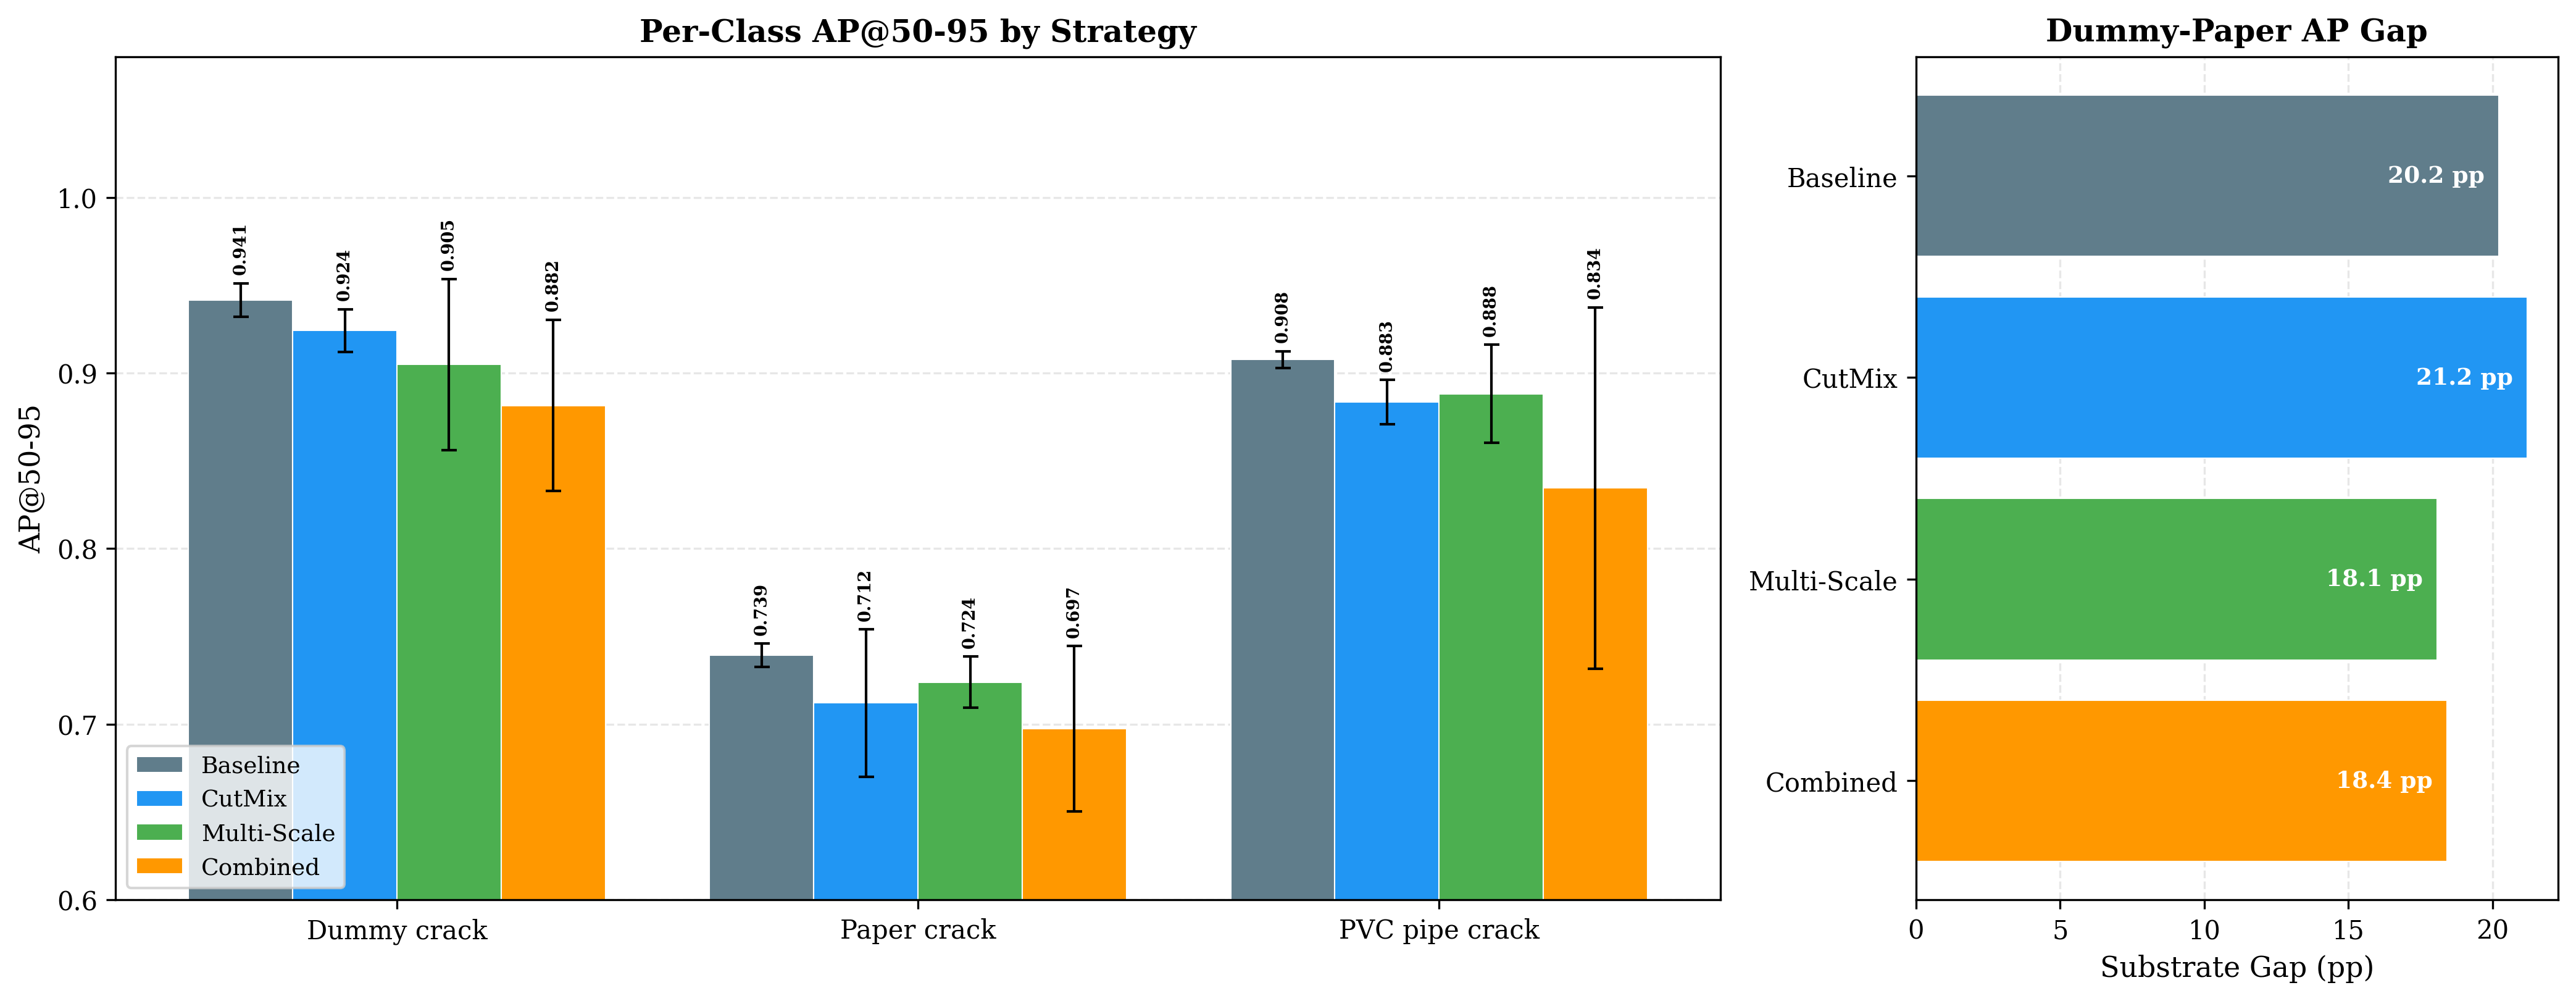
\includegraphics[width=\columnwidth]{fig_mitigation_comparison.png}}
\caption{Per-class AP@50-95 (left) and substrate gap (right) across mitigation strategies. The Dummy--Paper gap quantifies the substrate-dependent performance variation.}
\label{fig:mitigation}
\end{figure}

% ==============================================================
%   V. DISCUSSION
% ==============================================================
\section{Discussion}

\subsection{Substrate Complexity as the Governing Factor}

The results demonstrate that defect-substrate visual properties have a substantial effect on detection performance even when training data quantity is held constant. While the general principle that textured backgrounds degrade detection is established \cite{li2024texmsyolo, liu2023survey}, our contribution is to quantify this effect under controlled, class-balanced conditions and to show its consistency across architectures---demonstrating that the 20--22 percentage point AP gap cannot be dismissed as a data imbalance artifact. Both architectures produce the same performance hierarchy, governed by (1)~the signal-to-noise ratio between crack features and substrate texture, and (2)~the consistency of crack edge definition.

Comparing AP@50 with AP@50-95 reveals that the substrate effect is primarily a \textit{localization} problem (Fig.~\ref{fig:perclass_ap}). Paper crack maintains high AP@50 (97.2\%) but drops to 73.9\% at AP@50-95---a 23.3~pp localization gap. By contrast, dummy crack shows only a 5.3~pp gap (99.5\% to 94.2\%). This indicates that the model detects paper cracks reliably but cannot draw tight bounding boxes on textured backgrounds, where crack edges blend into the substrate. Practitioners should therefore account for substrate properties when estimating expected performance and may need targeted strategies such as hard-example mining or substrate-specific augmentation for visually complex categories.

\begin{figure}[htbp]
\centerline{
\includegraphics[width=\columnwidth]{fig_perclass_ap.png}}
\caption{Per-class AP at IoU thresholds 0.50 and 0.50--0.95 (YOLO-World XL, mean of 5 seeds). The gap between paired bars quantifies the localization penalty: paper crack drops 23.3~pp from AP@50 to AP@50-95, versus only 5.3~pp for dummy crack.}
\label{fig:perclass_ap}
\end{figure}

\subsection{Effectiveness of Augmentation-Based Mitigation}

The failure of all three augmentation strategies to close the substrate-dependent AP gap suggests that the performance disparity is not primarily caused by insufficient scale or appearance diversity during training. Instead, the gap likely reflects a more fundamental challenge: paper crack annotations exhibit inherently lower contrast and less distinctive boundary features, making precise localization difficult regardless of augmentation.

This interpretation is supported by two observations. First, the localization gap (AP@50 minus AP@50-95) for Paper crack is substantially larger than for the other classes across all strategies (baseline: 23.3~pp for Paper vs.\ 5.3~pp for Dummy and 8.4~pp for PVC), indicating that the detector finds Paper crack objects but struggles to localize them precisely. Second, the Combined strategy degraded \textit{all} classes uniformly rather than selectively improving Paper crack, with PVC pipe crack suffering the largest absolute drop ($-7.3$~pp), suggesting that aggressive augmentation harms fine-grained localization across the board. Addressing the substrate gap may therefore require strategies beyond training-time augmentation, such as substrate-specific fine-tuning, domain adaptation, or improved annotation protocols for low-contrast substrates.

\subsection{Transfer Learning Effectiveness}

YOLO-World's CLIP-based pre-training provides a measurable advantage (mAP@50-95 of $0.8628 \pm 0.0044$ vs.\ $0.8545 \pm 0.0075$), but the benefit was not uniform: pre-trained features transferred most effectively to high-contrast defects on smooth surfaces (94.2\% AP for YOLO-World XL and 94.0\% for YOLOv8x on dummy crack) and least to defects on textured substrates (73.9\% and 72.4\%, respectively, for paper crack). This indicates a fundamental visual domain challenge rather than a model-specific limitation.

\subsection{Limitations}

Several limitations bound generalizability. Dummy cracks are synthetic markings rather than physical defects, and paper cracks are formed on tissue rolls rather than pipe material; both represent controlled proxies for defect-substrate combinations rather than direct analogues of field conditions. Additionally, because crack generation methods differ across the three classes (drawn, physically induced, and formed on porous material), substrate texture and crack morphology are confounded. Annotation consistency may also play a role: bounding box placement on textured tissue is inherently more ambiguous than on smooth PVC, so part of the AP@50-95 gap may reflect ground-truth noise rather than model error. All specimens share a blue color, and only two single-stage YOLO architectures were compared. Extending to architecturally distinct detectors (e.g., Faster R-CNN, RT-DETR), naturally occurring defects, and diverse pipe materials would strengthen these conclusions.

% ==============================================================
%   VI. CONCLUSION AND FUTURE WORK
% ==============================================================
\section{Conclusion and Future Work}

This paper investigated how substrate visual complexity affects crack detection performance under controlled data conditions. A fine-tuned YOLO-World XL model achieved a mean mAP@50-95 of $0.8628 \pm 0.0044$ and F1 of $0.9826 \pm 0.0040$ over five seeds, yet per-class AP ranged from 94.2\% on smooth PVC to 73.9\% on textured tissue despite identical label counts of 400 per class. A parallel comparison with YOLOv8x confirmed that the substrate-dependent gap is consistent across the two architectures evaluated, with both models exhibiting a 20--22 percentage point performance hierarchy. Three augmentation-based mitigation strategies (CutMix, multi-scale training, and their combination) were further evaluated, but none significantly reduced the substrate gap (Bonferroni-corrected $p > 0.05$ for all comparisons), with the Combined strategy actually degrading overall mAP by 5.8~pp. The persistence of the gap under diverse augmentation conditions reinforces its origin as a fundamental localization challenge tied to substrate visual properties. These results demonstrate that defect-substrate visual properties, rather than data quantity or model choice, strongly influence detection difficulty.

Future work includes validating on naturally occurring pipe failures in field conditions, expanding to diverse pipe materials and architecturally distinct detectors (e.g., two-stage and transformer-based models), varying substrate properties while holding the crack formation mechanism constant to disentangle texture from morphology, and exploring targeted mitigation approaches such as substrate-specific fine-tuning, domain adaptation, or improved annotation protocols for low-contrast substrates---given that standard augmentation proved insufficient. The best-performing model can also be integrated into a mobile robotic platform for autonomous pipe inspection, building on prior work in differential drive trajectory optimization \cite{dimalanta2022trajectory}.

% ==============================================================
%   DATA AND CODE AVAILABILITY
% ==============================================================
\subsection*{Data and Code Availability}
The pipe crack detection dataset is publicly available on Roboflow Universe (\url{https://universe.roboflow.com/gazxard/pipe-crack-detection/dataset/1}) under a CC~BY~4.0 license. The training and evaluation code, including the multi-seed runner and analysis scripts, will be released at \url{https://github.com/gazzard-ust/pipe-crack-detection} upon publication.

% ==============================================================
%   ACKNOWLEDGMENT
% ==============================================================
\section*{Acknowledgment}
The authors used Claude (Anthropic) for manuscript editing and grammar refinement. All experimental design, data collection, model training, and analysis were performed by the authors.

% ==============================================================
%   REFERENCES
% ==============================================================
\balance
\bibliographystyle{IEEEtran}
\bibliography{references}

\end{document}